\documentclass[dvipdfmx,11pt]{beamer}
\usepackage{bxdpx-beamer}% dvipdfmxなので必要
\usepackage{pxjahyper}% 日本語で'しおり'したい
\usepackage{amsmath, amssymb, amsthm}
\usepackage{graphicx}
\usepackage{ulem}
\usepackage{wrapfig}
\usepackage{bbm}

\renewcommand{\kanjifamilydefault}{\gtdefault}% 既定をゴシック体に

\usetheme{TsukubaMin}

\theoremstyle{definition}
\newtheorem{defn}{定義}
\newtheorem{theo}{定理}
\newtheorem{propo}{命題}
\newtheorem{alg}{アルゴリズム}
\newtheorem{prob}{問題}

\makeatletter
\newenvironment{prooff}[1][\proofname]{\par
  \normalfont
  \topsep6\p@\@plus6\p@ \trivlist
  \item[\hskip\labelsep{\bfseries #1}\@addpunct{\bfseries.}]\ignorespaces
  \par
}{%
  \endtrivlist
}
\renewcommand{\proofname}{証明}
\makeatother

%タイトル
\title{クラスタリングで音楽が見れる!}
\subtitle{spectral graph theoryで音楽の構成を \\ 見よう}
\author{閔 正媛}
\date{2017/12/dd}
\begin{document}
\begin{frame}
	\titlepage
\end{frame}

\begin{frame}{Contents}
\begin{itemize}
\item はじめに
\item クラスタリングについて
\item グラフの話: 実はグラフを行列にして計算できるとか
\item Spectral graph theory
\item 中南米音楽について
\item 具体的な実装・楽曲の構成
\end{itemize}
\end{frame}

\section{はじめに}
\begin{frame}{自己紹介}
\begin{itemize}
\item 1988年 韓国ソウル生まれ
\item 2007年 筑波大学理工学群数学類入学
\item 2011年 筑波大学卒業 \\ 
\hspace{1.45cm} 東京工業大学大学院理工学研究科数学専攻入学
\item 2016年 博士学位取得(理学) \\ 
\hspace{1.45cm} システム計画研究所入社 \\ 
\item 実は中1から数学が好きでした\textcolor{gray}{\scriptsize \sout{(それで博士まで行きましたが, あまりの厳しさに研究者の夢なんか諦めてます, てゆーかそれだけじゃないっすけど)}}
\item 大学1年の頃から中南米音楽やってます \textcolor{gray}{\scriptsize \sout{(一緒にやる人がいなくて, 細々と練習を続けています \& こんな分析に走ってたりします)}}
\end{itemize}
\end{frame}

\vspace{6pt}
\begin{frame}{音楽の構成を数学で見るんですか?}
参考にした論文は \\
\vspace{6pt} 
Brian McFee and Daniel P.W.Ellis 著, Analyzing song structure with spectral clustering, ISMIR 2014 \\ 
\vspace{6pt}
です. \\ 
\vspace{6pt}
この論文に, クラスタリングを使って楽曲の構成(例えば$2:00 \sim 2:20$がサビだとか)を自動抽出するアルゴリズムについて議論されています.
\end{frame}

\section{クラスタリングについて}
\begin{frame}{クラスタリングとは}
クラスタリングとは, データをいくつかのクラスター(データの塊)で分割していく手法です. ラベルが付いていないデータを, 距離などを用いて分割していきますので, ラベルなしデータの解析に有効です. 
\begin{center}
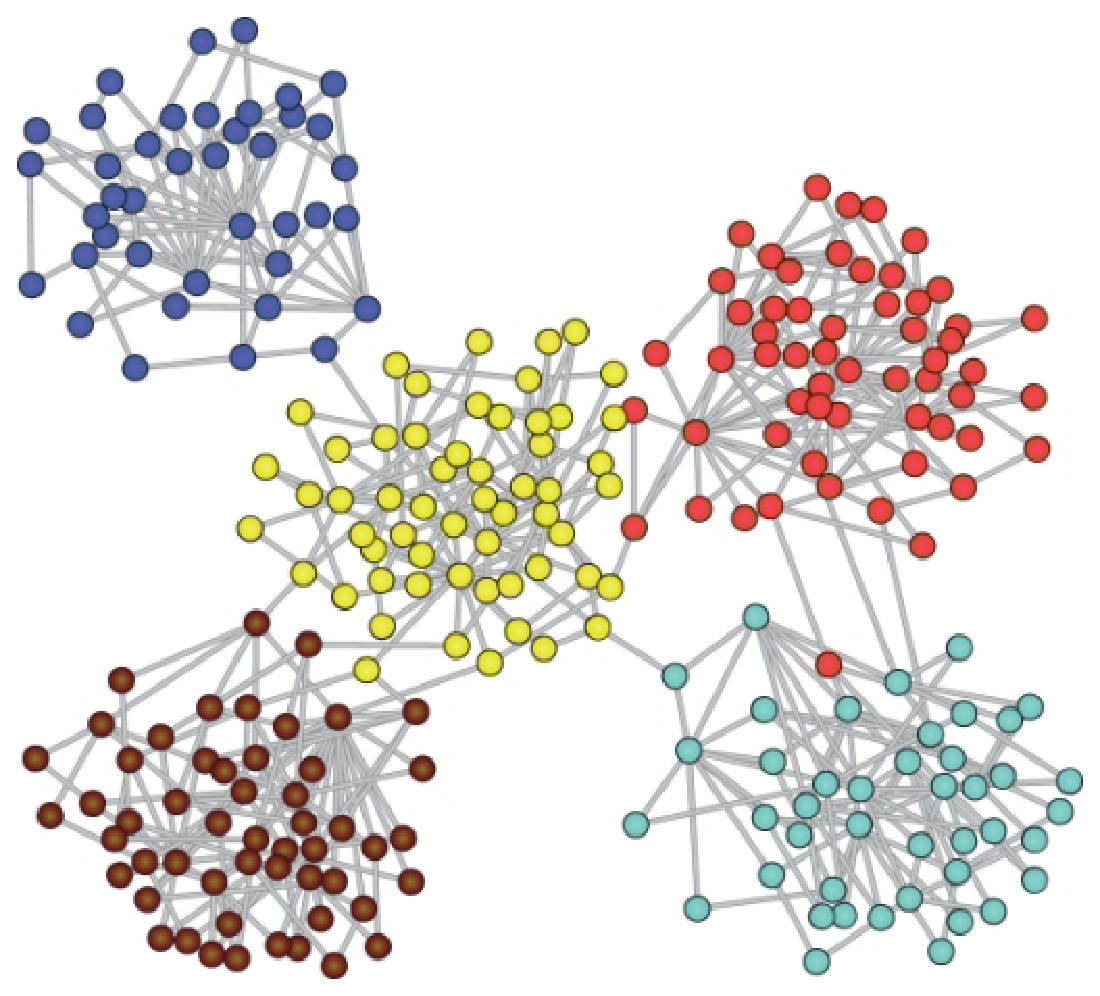
\includegraphics[width=6cm]{images/cluster_graph.eps}
\end{center}

\end{frame}

\begin{frame}{学習のはなし - コンピュータが学習するの?}
コンピュータがある仕組みによってデータの特徴を抽出していくことを「学習」と言います. 学習には, 次の2つの方法があります.
\begin{itemize}
\item 教師あり学習: すでにラベルが振ってあるデータからラベルごとの特性を学んでいくことです. \

\hspace{0.5cm} 例) SVM, Deep Learningなど
\item 教師なし学習: ラベルがないデータから特性を学び, データを分類していくことです. \

\hspace{0.5cm} 例) クラスタリングなど
\end{itemize}
\end{frame}

\section{グラフについて}
\begin{frame}{グラフ}
実は, "グラフ"と一口で言っても, グラフには2種類あります.
\begin{enumerate}
\item 関数$f : \, x \mapsto y$が与えられたとき, $(x,\,y)$の対, またはそれを可視化したものをグラフという. \\ 
(中1のころ"グラフは集合だ"という話を聞いてすごくショックを受けた記憶が未だに鮮明だったりする)
\item 頂点集合とエッジ(頂点と頂点をつなげるもの. 日本語では"辺"ともいう)集合の対. \label{2_graph}
\end{enumerate}
今回話す内容は, \ref{2_graph}のことです.
\begin{figure}
  \hbox{
    \hspace{-0.5cm}
    \begin{beamercolorbox}[wd=.5\paperwidth, right]{}
    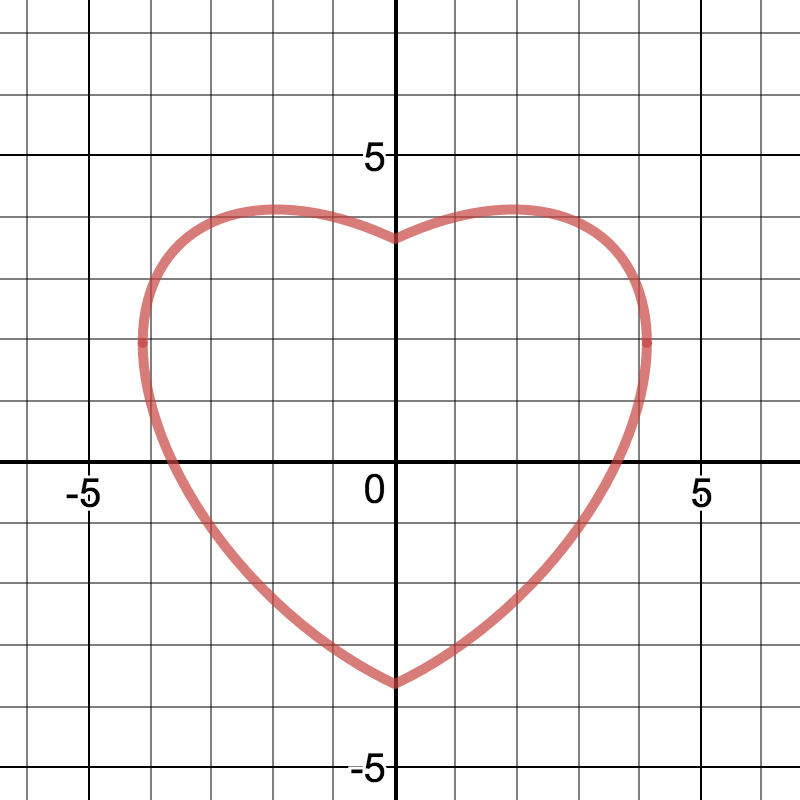
\includegraphics[height=3.5cm]{images/love_equation.png}
    \end{beamercolorbox}
    \begin{beamercolorbox}[wd=.5\paperwidth, left]{}
    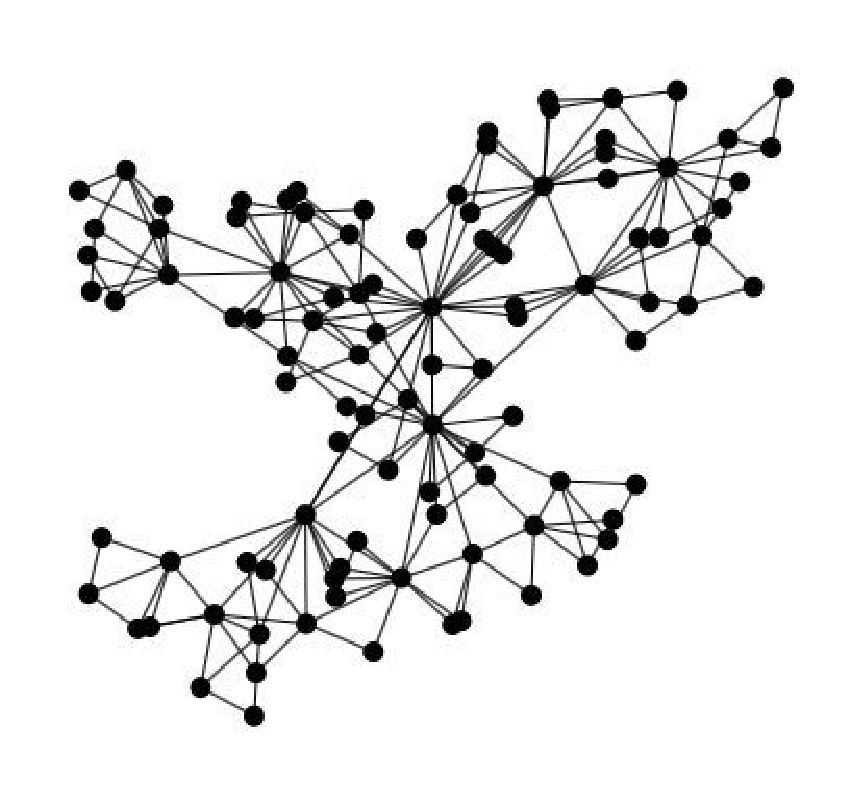
\includegraphics[height=3.5cm]{images/graph_theory.eps}
    \end{beamercolorbox}
  }
\end{figure}
\end{frame}

\section{グラフの話: 実は行列にして計算できるとか}
\begin{frame}{グラフを行列にしていろんな計算ができる}
今ノードに番号をつけていますが, その番号をそれぞれ縦と横で並べ, 間にエッジを挟むなら1, そうでなければ0を振っていきながら行列を作ります. \\ 

\begin{minipage}[c]{.35\textwidth}
 \begin{center}
  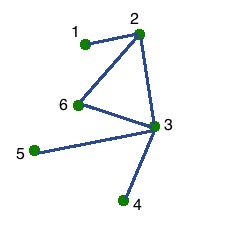
\includegraphics[width=\textwidth]{images/graph_to_matrix.png}
 \end{center}
\end{minipage}
\begin{minipage}[c]{.6\textwidth}
行列ならコンピュータに入力できますし, またこの行列からいろんな情報が見出せるので, 便利でもあり重要でもあります.
$$\begin{pmatrix}
0 & 1 & 0 & 0 & 0 & 0 \\
1 & 0 & 1 & 0 & 0 & 1 \\
0 & 1 & 0 & 1 & 1 & 1 \\
0 & 0 & 1 & 0 & 0 & 0 \\
0 & 0 & 1 & 0 & 0 & 0 \\
0 & 1 & 1 & 0 & 0 & 0 
\end{pmatrix}$$
\end{minipage}
\end{frame}

\begin{frame}{用語/記号など}
グラフの行列をどのように見ていくかの話をする前に、用語/記号から整理したいと思います。

\begin{minipage}[c]{.35\textwidth}
 \begin{center}
  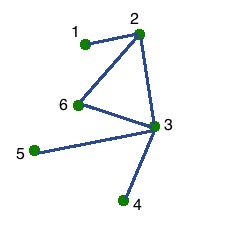
\includegraphics[width=\textwidth]{images/graph_to_matrix.png}
 \end{center}
\end{minipage}
\begin{minipage}[c]{.6\textwidth}
\begin{itemize}
\item ノードの集合を$V$, エッジの集合を$E$と書きます. 
\item グラフを$G = (V, E)$のように, ノードとエッジのタプルで表します. 
\item 1つのノードのつながっているエッジの本数を次数と言います. \\
各ノードの次数が対角線上に並んでいる対角行列を$D$と書きます.
\end{itemize}
\end{minipage}

\end{frame}

\section{Spectral graph theory}
\begin{frame}{グラフの行列とその固有値}
グラフの行列の固有値は, ノードの番号のつけ方によらないので, 大変重要な不変量の一つです. \\ 
例) ノード3つ, エッジ2本のグラフの場合
\begin{table}[h]
\begin{tabular}{ccc}
$\begin{pmatrix}
0 & 1 & 1 \\
1 & 0 & 0 \\
1 & 0 & 0
\end{pmatrix},$ & 
$\begin{pmatrix}
0 & 1 & 0 \\
1 & 0 & 1 \\
0 & 1 & 0 
\end{pmatrix},$ & 
$\begin{pmatrix}
0 & 0 & 1 \\ 
0 & 0 & 1 \\
1 & 1 & 0 
\end{pmatrix}$ 
\end{tabular}
\end{table}
この3つの行列の固有方程式はすべて$x^3 - 2x$です. \\ 
\vspace{0.4cm}
グラフの行列そのものではなく, ラプラシアン\textcolor{red}{$L = D - A$}や, 正規化されたラプラシアン\textcolor{red}{$L = I - D^{-1/2}A D^{-1/2}$}の固有値を見る場合もあります.
\end{frame}

\begin{frame}{重み付きグラフ}
"重み付きグラフ"の話をしましょう. \\ 

\begin{minipage}[c]{.45\textwidth}
 \begin{center}
  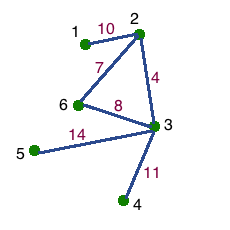
\includegraphics[width=40mm]{images/graph_to_matrix_weight.png}
 \end{center}
\end{minipage}
\begin{minipage}[c]{.45\textwidth} 
\begin{center}
$\begin{pmatrix}
 0 & 10 &  0 &  0 &  0 & 0 \\
10 &  0 &  4 &  0 &  0 & 7 \\
 0 &  4 &  0 & 11 & 14 & 8 \\
 0 &  0 & 11 &  0 &  0 & 0 \\
 0 &  0 & 14 &  0 &  0 & 0 \\
 0 &  7 &  8 &  0 &  0 & 0 
\end{pmatrix}$
\end{center} 
\end{minipage}

重みがついていないグラフは, すべてのエッジの重みが$1$のグラフとして考えられます.

\end{frame}

\begin{frame}{グラフの切断(カット)}

\begin{defn}
グラフ$G=(V, E)$について, $V$の分割, つまり$A, B\subset V,\,A \cap B = \phi,\, A\cup B = V$をみたす$V$の部分集合の対$(A,B)$を切断という.

また, 集合$A,\,B$をまたがるエッジの重みの総和を$W(A, B)$と書く. つまり, $$W(A, B) = \displaystyle\sum _{i \in A, \,j \in B} w_{ij},$$
ただし$w_ij$は$i$と$j$を結ぶエッジの重みである. 
\end{defn}

注意)

グラフの固有値とその重複度は, 頂点の番号のつけ方によらないので, この発表では頂点の集合と頂点につけた番号の集合を同一視する.
\end{frame}

\begin{frame}{グラフの切断}
\begin{minipage}[c]{.35\textwidth}
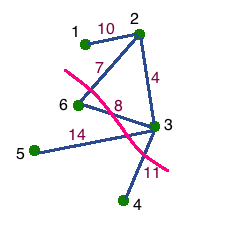
\includegraphics[width=\textwidth]{images/graph_cut.png}
\end{minipage}
\begin{minipage}[c]{.6\textwidth}
例えば, 左のグラフで切断$(A, B)$を$$A=\{1,2,3\}, B=\{4,5,6\}$$とすると, 
$$W(A,B)=7+8+14+11=40$$
となります.
\end{minipage}

\end{frame}

\begin{frame}{3つ以上の集合で分割する時のカットの考え方}
グラフの頂点をを3つ以上の集合$A_1, \cdots, A_k$で分割するとき, 次を考える.

\begin{minipage}[hc]{.25\textwidth}
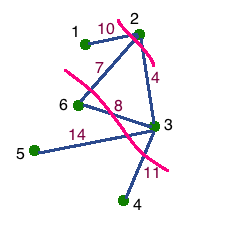
\includegraphics[width=\textwidth]{images/over2_cut.png}
\end{minipage}
\begin{minipage}[hc]{.7\textwidth}
\begin{enumerate}
\item すべての$W(A_i, A_j)$の和: 
\begin{equation*}
\scalebox{0.7}
{$\text{cut}(A_1,\cdots,A_k):= \dfrac{1}{2}\displaystyle\sum_{i=1} ^{k} W(A_i, A^c _i).$}
\end{equation*}
\item 次のような正規化を考えることもある.
\begin{enumerate}
\item RatioCut: 各分割の中の点の数で正規化
\begin{equation*}
\scalebox{0.8}
{$\text{RatioCut}(A_1,\cdots,A_k) := \dfrac{1}{2} \displaystyle\sum _{i=1} ^k \dfrac{W(A_i, A_i ^c)}{|A_i|} = \displaystyle\sum _{i=1} ^k \dfrac{\text{cut}(A_i, A_i ^c)}{|A_i|}.$}
\end{equation*}
\item Ncut: 分割された点集合の次数の総和で正規化
\begin{equation*}
\scalebox{0.8}
{$\text{Ncut}(A_1,\cdots,A_k):=\dfrac{1}{2} \displaystyle\sum _{i=1} ^k \dfrac{W(A_i, A_i ^c)}{\text{vol}(A_i)} = \displaystyle\sum _{i=1} ^k \dfrac{\text{cut}(A_i, A_i ^c)}{\text{vol}(A_i)}.$}
\end{equation*}
\end{enumerate}
\end{enumerate}
\end{minipage}
\end{frame}

\begin{frame}{グラフクラスタリングのアルゴリズム}
\begin{alg}[正規化なしの場合] 
\begin{enumerate}
\item 正規化なしラプラシアン$L$を求める.
\item ラプラシアン$L$の固有値を小さい順から$k$個求め, それらの固有ベクトル$u_1,\cdots,u_k$を求める. 
\item 固有ベクトル$u_1,\cdots,u_k$を縦に並べ, $U=[u_1,\cdots,u_k]= \mathbb{R} ^{n \times k}$を作る.
\item\label{clustering} $U$の各行をまたベクトルとして見て, $k$-meansを使ってクラスタリングを行う.
\end{enumerate}
\end{alg}
正規化されたラプラシアンをクラスタリングする場合は, \ref{clustering}でクラスタリングをする前に各行を正規化すればよい.
\end{frame}

\begin{frame}{ところで, なぜそのようにクラスタリングするの?}
いきなりラプラシアンの性質, 失礼します.
\begin{propo}
正規化なしラプラシアン$L = D - W$は次をみたす.
\begin{enumerate}
\item 任意のベクトル$f \in \mathbb{R}^n$について, 
$$^{t}f L f = \dfrac{1}{2}\displaystyle\sum _{i, j=1} ^n w_{ij} (f_i - f_j)^2$$
が成り立つ.
\item $L$は対称行列であり, positive semi-definiteである.
\item $L$の最小の固有値は$0$であり, 対応する固有ベクトルは$\mathbbm{1}$である.
\item $L$は非負な実数固有値$0 =\lambda _1 \leq \lambda_2 \leq \cdots \lambda_n$ をもつ.
\end{enumerate}
\end{propo}

\end{frame}

\begin{frame}{証明}

\begin{prooff}


\begin{enumerate}
\item \label{sym}$L$の定義より, 次が成り立つ.
\begin{equation*}
\begin{split}
^{t}f Lf &= ^{t}fDf - ^{t}fWf = \displaystyle\sum _{i=1} ^n d_i f_i ^2 - \displaystyle\sum _{i,\,j=1} ^n f_i f_j w_ij \\
&= \dfrac{1}{2} \biggl( \displaystyle\sum _{i=1} ^n d_i f_i ^2 - \displaystyle\sum _{i,\,j=1} ^n f_i f_j w_{ij} + \displaystyle\sum _{j=1} ^n d_j f_j ^2 \biggr) = \dfrac{1}{2} \displaystyle\sum _{i,\,j=1} ^n w_{ij} (f_i - f_j)^2.
\end{split}
\end{equation*} 
\item $D$, $W$ともに対象なので$L$も対象. positive semi-definiteは\ref{sym}より.
\item すぐわかる. ($D$が$W$の各行の話を対角線上に並べたやつということからすぐわかる)
\item 上の3つから導かれる.
\end{enumerate}
\end{prooff}

\end{frame}

\begin{frame}{正規化されてラプラシアンについては}

\begin{propo}
\begin{enumerate}
\item 任意の$f \in \mathbb{R}^n$について,
$$^{t}f L f = \dfrac{1}{2} \displaystyle\sum _{i,\,j=1} ^n w_{ij} \biggl( \dfrac{f_i}{\sqrt{d_i}} - \dfrac{f_j}{\sqrt{d_j}} \biggr)^2$$
が成り立つ.
\item $0$は$L$の固有値であり, 付随する固有ベクトルは$D^{1/2} \mathbbm{1}$となる.
\item $L$はpositive semi-definiteであり, $n$個の非負な実数固有値$0 = \lambda _1 \leq \cdots \leq \lambda_n$をもつ.
\end{enumerate}
\end{propo}

証明は割愛します.

\end{frame}

\begin{frame}{クラスタリングのアルゴリズム(再)}

\begin{alg}[正規化なしの場合] 
\begin{enumerate}
\item 正規化なしラプラシアン$L$を求める.
\item ラプラシアン$L$の固有値を小さい順から$k$個求め, それらの固有ベクトル$u_1,\cdots,u_k$を求める. 
\item 固有ベクトル$u_1,\cdots,u_k$を縦に並べ, $U=[u_1,\cdots,u_k]= \mathbb{R} ^{n \times k}$を作る.
\item\label{clustering2} $U$の各行をまたベクトルとして見て, $k$-meansを使ってクラスタリングを行う.
\end{enumerate}
\end{alg}
正規化されたラプラシアンをクラスタリングする場合は, \ref{clustering2}でクラスタリングをする前に各行を正規化すればよい.

\end{frame}

\begin{frame}{アルゴリズムの解説}

次の問題を考えましょう.
\begin{prob}
RatioCutを最小にする分割$(A, A^c)$を求めるには?
\end{prob}

ある部分集合$A \subset V$について, 次のベクトル$f \in ^{t}(f_1, \cdots, f_n) \in \mathbb{R}^n$を考えよう.
$$f_i =
\begin{cases}
\sqrt{|A^c| / |A|} & \text{if }v_i \in A, \\ 
-\sqrt{|A| / |A^c|} & \text{if } v_i \in A^c .
\end{cases}$$

このとき, 正規化なしラプラシアン$L$について次を得る.

(次のページにつづく)
\end{frame}

\begin{frame}

\begin{equation*}
\scalebox{0.7}
{$\begin{split}
^{t}f L f &= \dfrac{1}{2} \displaystyle\sum _{i,\,j = 1} ^n w_{ij} (f_i - f_j)^2 \\ 
&=\dfrac{1}{2}\displaystyle\sum _{i\in A,\, j \in A^c} w_{ij} \biggl(\sqrt{\dfrac{|A^c|}{|A}} + \sqrt{\dfrac{|A|}{|A^c|}} \biggr)^2 + \dfrac{1}{2} \displaystyle\sum _{i \in A^c, \,j \in A} w_{ij} \biggl(-\sqrt{\dfrac{|A^c|}{|A|}} - \sqrt{\dfrac{|A|}{|A^c|}} \biggr)^2 \\ 
&= \text{cut}(A, A^c)\biggl(\dfrac{|A^c|}{|A|} + \dfrac {|A|}{|A^c|} + 2 \biggr) \\ 
&= \text{cut}(A, A^c)\biggl(\dfrac{|A|+ |A^c|}{|A|} + \dfrac{|A|+|A^c|}{|A^c|} \biggr) \\ 
&= |V| \cdot \text{RatioCut}(A, A^c).
\end{split}$}
\end{equation*}
特に
\begin{equation*}
\scalebox{0.7}
{$\displaystyle\sum _{i=1} ^n f_i = \displaystyle\sum_{i \in A} \sqrt{\dfrac{|A^c|}{|A|}}-\displaystyle\sum_{i \in A^c} \sqrt{\dfrac{|A|}{|A^c|}} = 0,$}
\end{equation*}
\begin{equation*}
\scalebox{0.7}
{$ \parallel f \parallel ^2 = \displaystyle\sum _{i=1} ^n f_i ^2 = |A|\dfrac{|A^c|}{|A|} + |A^c|\dfrac{|A|}{|A^c|} = n $}
\end{equation*}
より, この問題は次の問題に帰着する.
\begin{equation*}
\scalebox{0.7}
{$f \perp \mathbbm{1}\text{であり, }
\min _{A \subset V} {}^{t}fLf, \,
\parallel f \parallel =\sqrt{n}$}
\end{equation*}
となるように$f$の成分を分けよう.
\end{frame}

\begin{frame}{音楽をどうやってグラフにするの?}
\begin{enumerate}
\item 音楽を取り込む: constant-Q(C2$\sim$C8)と最初の13 Mel frequency cepstral coefficients(MFCC)を取り込む

(python librosaで, 音楽を行列の形で取り込むことができる)
\item\label{label2} beatで区切って平均を算出し, 取り込んだ音楽の行列を圧縮する(これもlibrosaでできる)
\item \ref{label2}で取り込んだ行列 $X=\begin{bmatrix}x_1, x_2, \cdots, x_n \end{bmatrix} \in \mathbb{R}^{d\times n}$($n$が時間軸. 実装上は転置を行う必要がある)について, 次のような行列を構成する.
$$R_{ij}(X) := 
\begin{cases}
1 & x_i, x_j \text{は互いに}k\text{-nearest} \\
0 & \text{otherwise}
\end{cases}$$
($k$については後述)
\item 行列$R$の各成分の周りの対角成分を見て, $0$と$1$のうち多い方を選んで$R^{\prime}$を作る.

(行列$R$をなだらかにする作業らしい)

\end{enumerate}
\end{frame}

\begin{frame}{音楽のグラフ(続き)}
近いベクトルだけでなく, 隣り合ったベクトルという要素も加味して, 次のように"無向グラフ"を作る.

$$ \Delta _{ij} :=
\begin{cases}
1 & |i - j | = 1 \\
0 & \text{else}
\end{cases}$$
とする. つまり, $i$, $j$が隣り合っていたら1, そうでなければ0ということ.
ここで, パラメータ$\mu \in [0, 1]$について,
$$R^{\mu} _{ij} := \mu R^{\prime} + (1-\mu)\Delta _{ij}$$
を考えよう. このパラメータを, だいたい
$$ \mu \displaystyle\sum _j R^{\prime} _{ij} \approx (1-\mu) \displaystyle\sum _j \Delta _{ij}$$
となるようにしておきたい. 
\end{frame}

\begin{frame}{音楽のグラフ}
グラフGの点iの次数の和を$d_i (G)$, つまり$d_i (G) := \sum _j G_{ij}$とする. このとき, 
$$\min _{\mu \in [0,1]} \dfrac{1}{2}\displaystyle\sum _i(\mu d_i (R^{\prime}) - (1 - \mu ) d_i (\Delta))^2$$ となる$\mu$を求めると, $\mu$は次のようになる.
$$ \mu = \dfrac{ \langle d(\Delta), d(R ^{\prime}) + d(\Delta) \rangle}{\| d(R ^{\prime}) + d(\Delta) \| ^2},$$
(ただし$d(\cdot) := [d(\cdot)]_{i=1} ^n$)となる.
\end{frame}

\begin{frame}{音楽のグラフ}
次に, $R^{\prime}$に対して, 次のように行列$S^{\text{rep}}$を求めて$R^{\prime}$をマスクする.
$$S^{\text{rep}} _{ij} := \exp \biggl( -\dfrac{1}{2 \sigma ^2} \| x_i - x_j \| ^2 \biggr),$$
ただし$\sigma ^2$は$x_i$ごとの$k$-nearestとの2乗距離の平均であり, $k$はbeat $n$について$1+\lceil \log _2 n \rceil$である.

また, MFCCについても, 同じ要領でガウシアンカーネル$S^{\text{loc}}$を求めておく.

ここまでできたら, 次のように音楽の(無向/重み付き)グラフ$A$を作る.
$$ A_{ij} := \mu R^{\prime} _{ij} S^{\text{rep}} _{ij} + (1-\mu) \Delta _{ij} S^{\text{loc}} _{ij}.$$
\end{frame}

\begin{frame}{中南米音楽について}
\begin{itemize}
\item 対象としている音楽は, アンデス山脈で伝承されている音楽を継承した民族音楽のジャンルである'フォルクローレ'
\item フォルクローレが演奏されている国は、ボリビア, ペルー, チリ, エクアドル, アルゼンチンなど数々の国
\item 基本的には, ケーナやサンポーニャといった管楽器と, ギターやチャランゴなどの弦楽器, その他様々なパーカッションで構成されている
\item 踊りと一緒に発展してきた総合芸術的な性格をもつ
\item 地形や地域の事情によって, 様々な様式の音楽が演奏されている
  \begin{itemize}
  \item ボリビアは国民性が比較的保守的だと言われていて, 楽器の構成もオーソドックスな構成を好むグループが多いよう
  \item エクアドルは, 欧米の影響をもっとも強く受けていて, バイオリンやマンドリンを積極的に取り入れている
  \end{itemize}
\end{itemize}
\end{frame}

\begin{frame}{中南米音楽奏者の事情いろいろ}
\begin{itemize}
\item 中南米音楽は歌と踊りが一緒になっている総合芸術なのに, 奏者の中には音楽しかできない人も多い
\item 五線譜に表現できないリズムもあるが, 音楽を習っている人たちはあらゆる音楽をまず五線譜から理解しようとする
\end{itemize}
$\rightarrow$ 違う紀元を持つ違う国の音楽を, ただリズムの刻み方が同じく聞こえるという理由だけで一色単にすることも多い

\begin{itemize}
\item エクアドルのサンファニートとボリビアのトバスを演奏するとき特に顕著(実際tobas-sanjuanitoも存在) 
\item 楽曲の構成の違いは聞いてわかる程度ではある(2, 3年目以上の熟練者の場合)
\end{itemize}
$\rightarrow$ サンファニートとトバスの可視化を通して, その違いをわかりやすくしてみたかった 
\end{frame}

\begin{frame}{サンファニートとトバスの違い}
\begin{itemize}
\item サンファニートは, 4小節程度の小さな"パーツ"(だいたい3, 4個程度)の繰り返しが3回以上繰り返されることもしばしばある
\item トバスは, "半分に分けるとだいたい同じ"場合が多い
\end{itemize}
\end{frame}

\begin{frame}{クラスタリングの例}
例をいくつかあげる.
\begin{itemize}
\item Purimuy (エクアドル伝統音楽/サンファニート)
\item Hija del Sol (アワティーニャス(ボリビア) / サンファニート)
\item Paloma Volvera (アワティーニャス(ボリビア) / トバス)
\end{itemize}
\end{frame}

\begin{frame}{クラスタリング結果を眺めて見て}
\begin{itemize}
\item $$\text{イントロ} - A\text{メロ} - A^{\prime}\text{メロ} - \text{イントロ} - B\text{メロ} - \cdots$$
といったパターンを自動的に検出して欲しかったけどな…

$\rightarrow$ Music annotationそのものについてもうちょっと研究する必要があるかもしれない 
\item しかし, 少なくとも"このパターンが頻繁に繰り返されている"などの可視化はできている感じ
\end{itemize}
\end{frame}

\begin{frame}{これからやりたいこと}
\begin{itemize}
\item プログラミングの基礎を固める: プログラミング言語のバックボーンとなっている数学(カテゴリー理論など)を勉強したい
\item 中南米音楽のアノテーションデータを構築し, それらを"言語"のように考えて正規表現的に分析したい(アイデアはあるが, アノテーションの基準をきちんと決めるなどといった細かいタスクが一杯残っている)
\end{itemize}
\end{frame}

\end{document}

